\mia{Will move stuff down to discussion, but simpler to write in the same section for now}

\subsection{Hyperparamters}

Through grid search the best combination of $\lambda$- and degree-values where found to be: 

\begin{table}[h!]
    \centering
    \begin{tabular}{|c|c|c|c|}
        \hline
        & & \textbf{Franke Function} & \textbf{Terrain Data} \\ \hline
        \textbf{Ridge} & $\lambda$ & 2.4 $\times 10^{-2}$ & 3.0 $\times 10^{-5}$ \\ 
         & degree & 7 & 4 \\ \hline
        \textbf{Lasso} & $\lambda$ & 1.7 $\times 10^{-5}$ & 2.2 $\times 10^{-4}$ \\ 
         & degree & 7 & 6 \\ \hline
    \end{tabular}
    \caption{Best pairs of $\lambda$- and degree values found through grid search}
    \label{tab:my_label}
\end{table}

\subsection{Franke function}

\begin{figure}[h!]
    \centering
    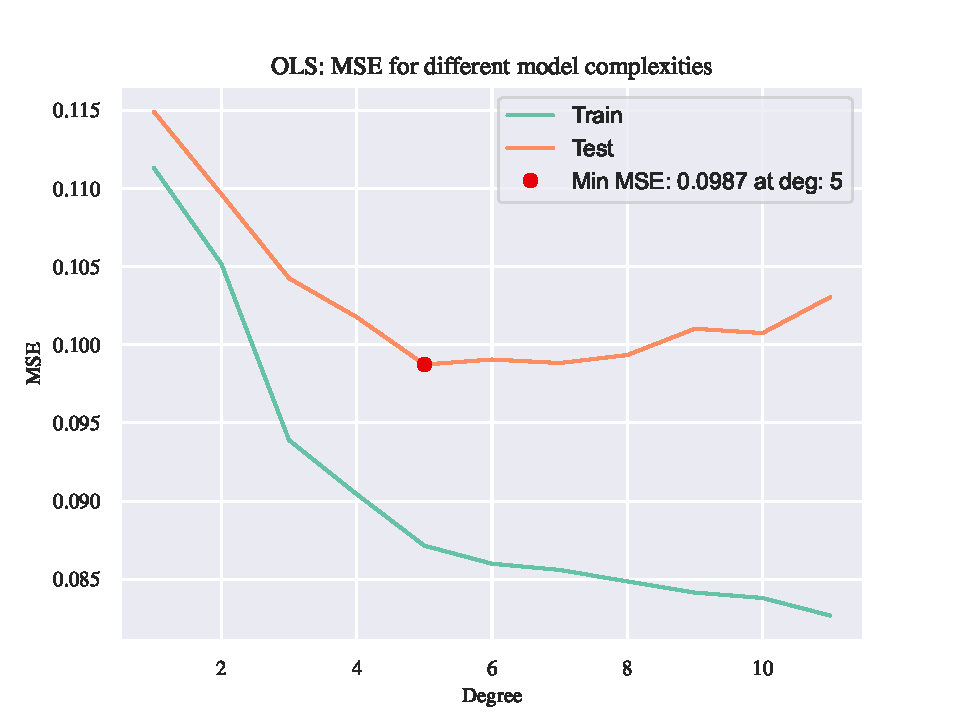
\includegraphics[width=1\linewidth]{project_1_alt/figures/figures_in_report/OLS_MSE_Franke_Noise.pdf}
    \caption{Caption}
    \label{fig:mseols}
\end{figure}

Fig. \ref{fig:mseols} shows how the error initially decreases as the degree of complexity increases. This seems reasonable as the Franke function makes up a complicated surface and one would think that higher degree polynomials are necessary to replicate it. 

We furthermore notice how at around degree = 9, the test error reaches its minimum. The error increases as the polynomial degree is increased by one. We use the test error to choose the optimal degree of complexity. In this case, polynomials of degree up to nine is the best. The training error continues to decrease. This is due to overfitting and the fact that OLS is designed to minimize the MSE. 

\begin{figure}[h!]
    \centering
    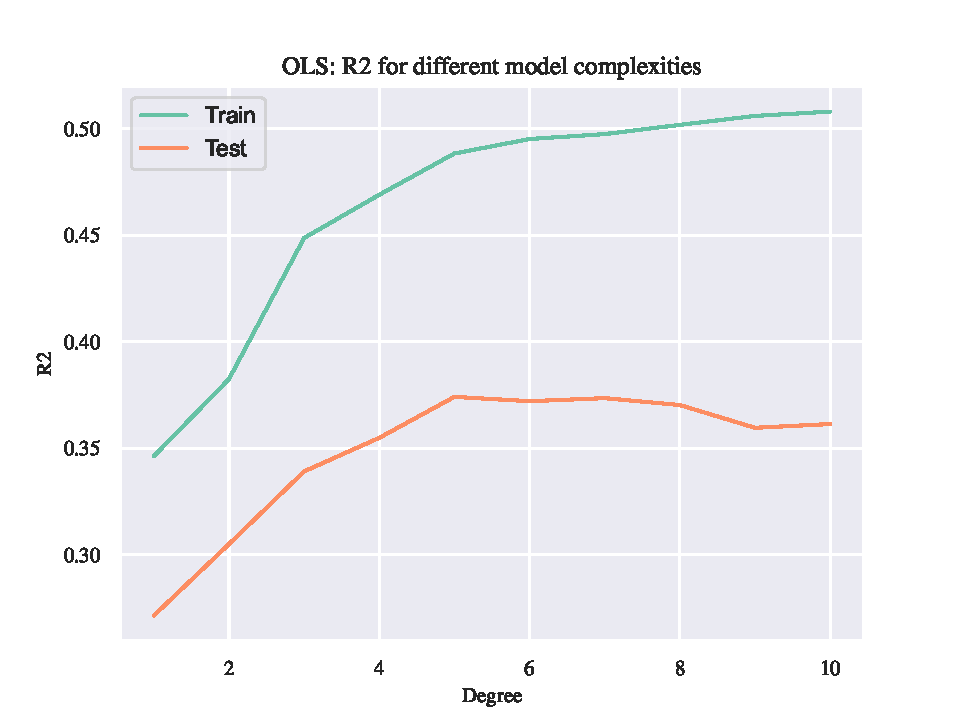
\includegraphics[width=1\linewidth]{project_1_alt/figures/figures_in_report/OLS_R2_Franke_Noise.pdf}
    \caption{Caption}
    \label{fig:r2ols}
\end{figure}

The $R^2$ value increases as higher degree polynomials are introduced to the ordinary least squares model, as shown in Fig. \ref{fig:r2ols}. This is reasonable as we likely need higher degree polynomials to explain more variance in the data. The increase in $R^2$ halters at around degree equal to 10. At this point, introducing higher degree polynoimals does not help explain further variance in the data. The value of $R^2$ for the test data is lower then the one for the training data. This might be a sign that the model does not generalize well. \mia{back this up}

\begin{figure}
    \centering
    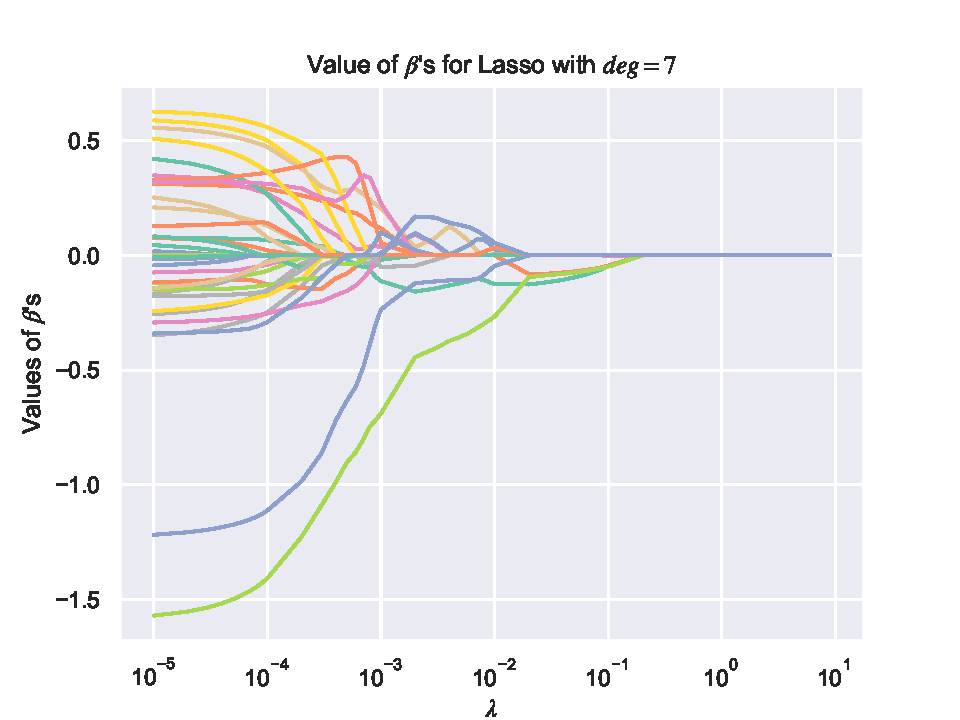
\includegraphics[width=1\linewidth]{project_1_alt/figures/figures_in_report/Ridge_Betas_lambda_Franke_Noise_const_deg.pdf}
    \caption{\mia{Caption}}
    \label{fig:ridge_betas}
\end{figure}

\begin{figure}
    \centering
    \includegraphics[width=1\linewidth]{project_1_alt/figures/figures_in_report/.pdf}
    \caption{\mia{caption}}
    \label{fig:lasso_betas}
\end{figure}

The $\beta$'s values for our Ridge- and Lasso regression models are presented in fig. \ref{fig:ridge_betas} and fig. \ref{fig:lasso_betas} respectfully. For both models, we observe that the values of the coefficients are forced towards zero, and thereby also each other, as the penalty increases. For the Ridge regression coefficients, all have non-zero values regardless of the size of the penalty. For Lasso regression however, we observe that some are brought to zero at a sufficiently large penalty. Closer to $\lambda = 10^0 = 1$ all values of the $\beta$'s are brought to zero. 


\mia{ comparing bootstrap to cross validation for franke function here}

\mia{discussion on the choice of K}

\begin{figure}[h!]
    \centering
    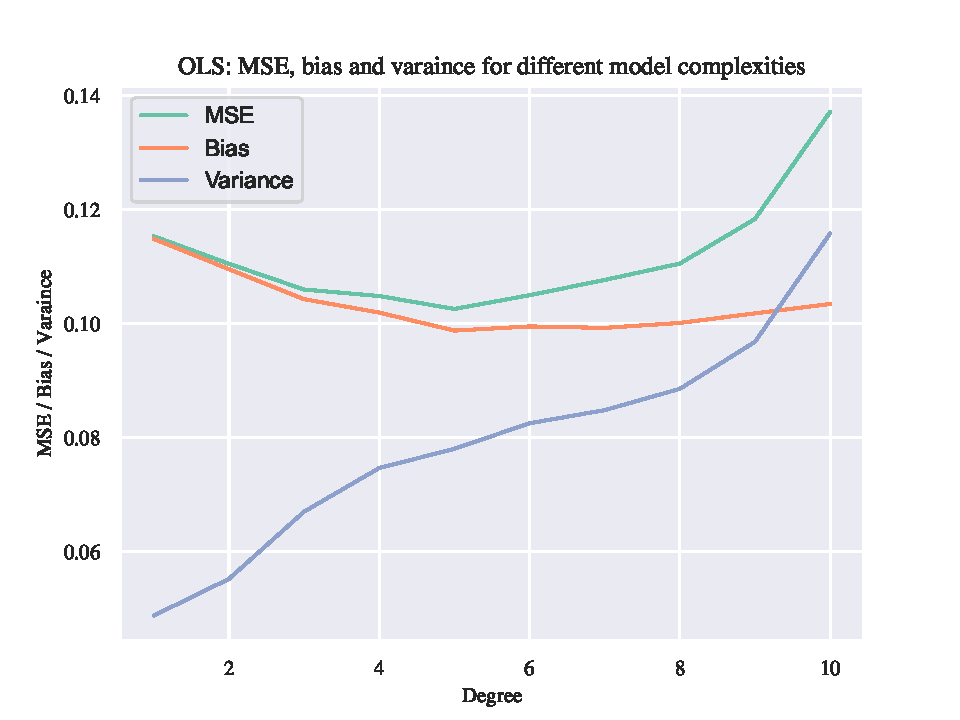
\includegraphics[width=1\linewidth]{project_1_alt/figures/figures_in_report/bias_var_Franke_Noise_bootstrap.pdf}
    \caption{caption}
    \label{bias_var_trade}
\end{figure}

For the OLS model trained with bootstrapping, fig. \ref{bias_var_trade} shows how the MSE can be decomposed into a bias and a variance term. The bias is initially high, but the variance is low. This is typical for an underfitted model. As the complexity is increases, the bias goes down, whereas the variance increases. The lowest MSE is reached at some trade-off between the two. In our case the minimal MSE is found at \mia{insert}. As the model complexity is further increased, the variance substantially increases and ensures an even higher MSE than at the beginning. This is a sign of a overfitted model.

\subsection{Terrain data}

\plothere{OLS, Ridge and Lasso for terrain data}

\begin{figure}[h!]
    \centering
    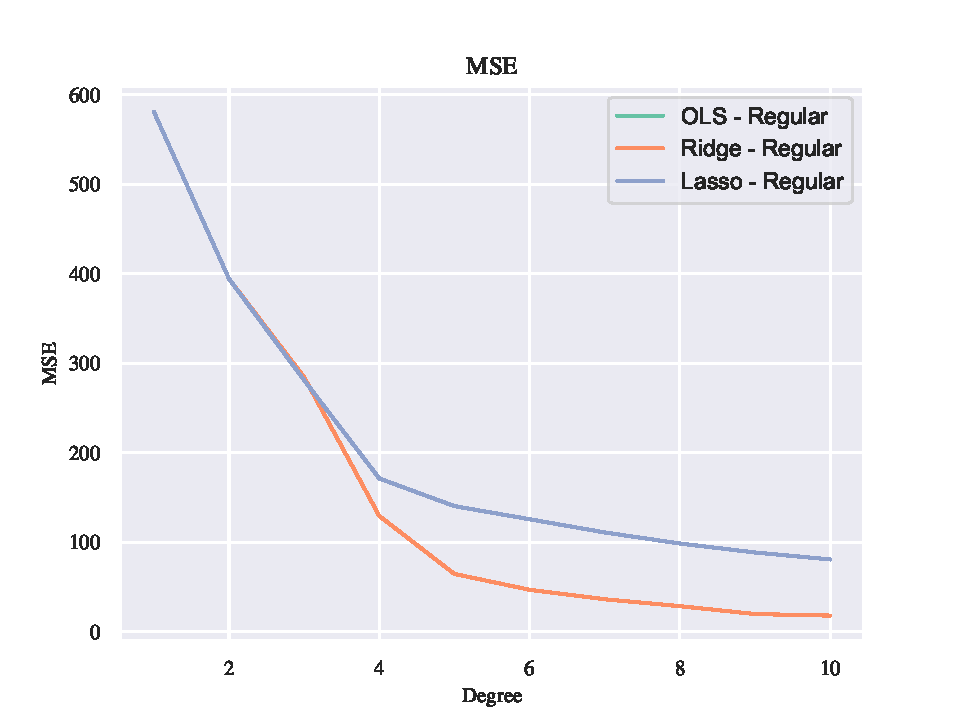
\includegraphics[width=1\linewidth]{project_1_alt/figures/figures_in_report/All_Terrain_OLS.pdf}
    \caption{caption}
    \label{bias_var_trade}
\end{figure}

\mia{which one is the best one, why might that be}

\plothere{OLS, Ridge and Lasso for terrain data with CV}
\begin{figure}[h!]
    \centering
    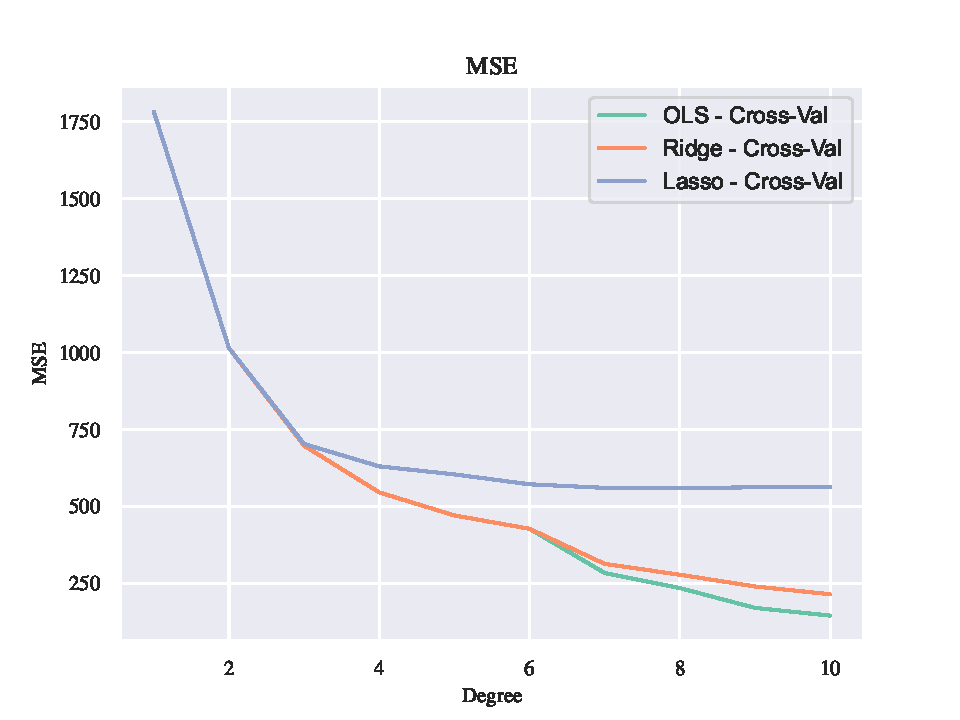
\includegraphics[width=1\linewidth]{project_1_alt/figures/figures_in_report/All_Terrain_CV_k10.pdf}
    \caption{caption}
    \label{bias_var_trade}
\end{figure}

\mia{which one is the best one, why might that be}

\plothere{OLS, Ridge and Lasso for terrain data with bootstrap}
\begin{figure}[h!]
    \centering
    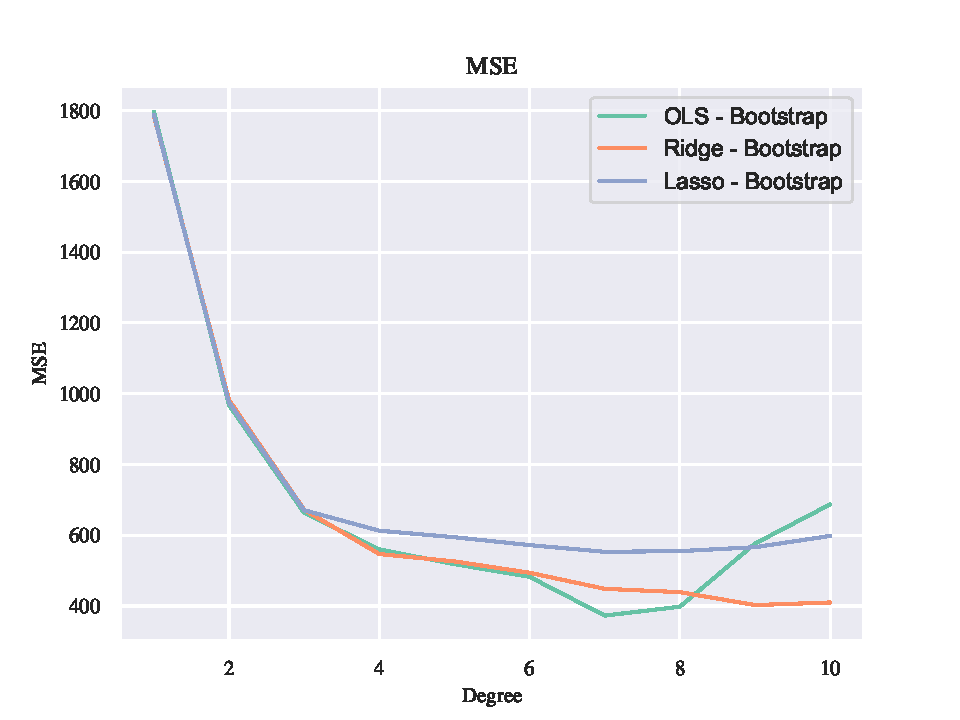
\includegraphics[width=1\linewidth]{project_1_alt/figures/figures_in_report/All_bootstrap_Terrain.pdf}
    \caption{caption}
    \label{bias_var_trade}
\end{figure}
\mia{which one is the best one, why might that be}

\mia{which one of the methods give the absolute lowest value for MSE -> our best method yey}

\mia{discussion of which to trust the most}

